
\begin{frame}{OCaml 5}


\begin{figure}
    \centering
    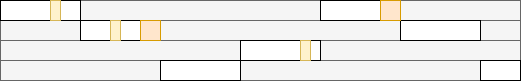
\includegraphics[width=0.9\textwidth]{slides/images/concurrence.png}
    \caption{Concurrence}
\end{figure}

\begin{figure}
    \centering
    \includegraphics[width=0.9\textwidth]{slides/images/parallélisme.png}
    \caption{Parallélisme}
\end{figure}
% Blanc = code OCaml
% Jaune = minor GC
% Orange = major GC
\end{frame}

\begin{frame}{Peterson}
    
\end{frame}

\begin{frame}{Lamport}
    
\end{frame}
